\chapter{地球系统模式面临的不确定性问题}
\label{cha:intro}

\section{论文的背景与意义}
2018年IPCC发布全球升温1.5摄氏度特别报告,报告指出,应该将全球变暖限制在1.5摄氏度,相比之前提出的限制在2摄氏度可以显著减少对气候变化的影响,而过去一个世纪,全球已升温1摄氏度,在全球变暖的背景下,寒潮、龙卷风、干旱、暴雨、暴雪,火灾等极端气候事件加剧。特别是近几年来,极端事件的频发,对人类的生命和财产都造成了不可挽回的损失。例如2016年我国暴雨频发,共出现46次区域暴雨,26个省(区、市)出现城市内涝;在非洲之角,2017年1月至2月严重的干燥季节以及3月至5月降雨极少的雨季,索马里超过半数的耕地遭受旱灾;2018年加利福尼亚遭受的毁灭性的野火是美国一个多世纪以来最致命的火灾。这些极端天气的出现,气候问题的逐渐凸显,如此现状为气候模拟预测提出了严峻的挑战。

地球系统模式作为模拟天气气候的数值模拟模型,是模拟预测未来气候的强有力的工具。它是通过建立数学物理方程组来模拟地球系统中大气、海洋、陆面、海冰和生态等各个圈层内的动力、物理和化学等复杂过程以及圈层间的水汽、能量和物质的交换过程。地球系统模式模拟的过程比一般气候系统模式更复杂,包括了大气环流、太阳辐射、陆面水文、植被、海洋海冰、气溶胶和人类活动等,地球系统模式模拟的准确性决定着气候预测的预报能力。

气候系统预测的不确定性是导致模拟不准确性的主要原因。其主要有地球系统模式的不确定性、温室气体等排放场景的不确定性,以及气候系统的内部变率的不确定性。IPCC会议对排放场景的不确定性的处理是设计多个排放场景,在不同的场景下对气候进行预测,对于内部变率的不确定性会随着模拟的时长而不断减少,所以目前亟待研究的是地球系统模式的不确定。地球系统模式的不确定性是气候模拟准确与否的决定性因素。地球系统模式的不确定性又分为模式结构的不确定性、边界条件不确定性、初始条件不确定性和物理参数不确定性。模式结构的不确定性是由于地球系统模式由大气、海洋、海冰、陆地等多个模块组成,每个模块都在不断的发展过程中,模式在构建的过程中也存在着大量的假设和近似操作,每个模块都还在研究之中,与真实的情况存在着巨大的差异,还有待深入的研究,理论也尚未成熟。边界的不确定性指的是模式的边界情况十分复杂,模拟的边界会对模拟产生巨大的影响,例如大气模式的下边界由地形状况、人类活动、生态环境等构成,而大气模式的上边界也包括太阳活动等。这上下边界都会对大气模式的模拟产生巨大的影响。初始条件的不确定性指的是气候模拟初始场的不确定性,由于洛伦兹提出的蝴蝶效应可知,初始场微小的差异将会引起模拟结果的不同,而物理参数化的不确定性则指的是地球系统模式中的物理参数化过程中存在着很多不确定性参数,这些参数是由专家根据经验而人为设定的,而地球系统模式的每个模块中都存在着大量的不确定性参数,这些不确定性参数也决定了模式准确性与否。

集合预报技术是一种针对地球系统模式不确定性分析的重要策略。其方法的原理是利用多个集合预测来代替原有的单一预报。集合预报已在各大预报中心得到应用。常用的方法有参数集合预报以及初值集合预报。
参数集合是
初值集合预报是

集合预报所面临的问题
(1)地球系统模式中的参数不确定性问题
(2)初值不确定性问题
(3)
本文主要关注的是初始条件的不确定性和物理参数的不确定性,这也是目前阶段最急需解决的不确定性问题。初始条件的不确定性的解决方案是利用同化和集合等方法。

当前针对不确定性分析的方法有前向的不确定性分析方法和反向的不确定分析方法。

\section{当前的不确定性分析方法}
\label{sec:first}
面对参数的不确定性问题,我们可以用现有的不确定分析方法。现有的不确定性分析方法主要分为前向的不确定性分析和反向的不确定性分析。下面将对这两类方法分别介绍

(1)	前向的不确定分析方法

前向的不确定性分析方法其核心思想是通过设计实验以及定量分析结果的统计特征等增加对问题本身的了解。主要的方法有采样、敏感性分析、构建代理回归模式等等。在不确定参数空间中进行采样,通过对采样点的评估,估计在参数空间中后验分布可能的分布情况。其方法可以是蒙特卡罗采样,单参数扰动采样,拉丁超立方采样,以及自适应采样等等。敏感性分析是指通过对参数的扰动来获取参数的灵敏度信息,如果一个参数扰动极小的幅度就会对评估结果产生较大的影响,那么就可以判定其为敏感参数。敏感性分析方法主要分为局部敏感性分析和全局敏感性分析。局部敏感性分析主要考虑的是参数的一阶效应。不考虑两个或多个参数之间的交互效应。而全局敏感性分析是要同时考虑一阶效应和交互效应的。一般在地球系统模式中参数之间的交互效应极为强烈的。构建代理模式是利用统计回归等方法构建类似原来复杂问题的简单模型,用简单模型代替复杂模型的运行。

(2)	反向的不确定性分析方法

反向的不确定性分析方法不考虑问题的统计特征,不要求对问题的后验分布有很好的了解,主要是通过每一次模型的运行结果与观测进行对比,用对比结果来指导下一次参数的取值。主要的方法是数值优化方法。数值优化方法有传统的优化方法有进化的优化方法等。传统的数值优化方法有单纯形下山方法、powell方法等等,这些方法是局部优化方法,其特点是优化速度很快,能够快速收敛,但是在复杂多维的问题下容易陷入局部最优。进化方法通过模拟种群进化的策略来不断更新样本,在种群中,根据物竞天择,适者生存的进化理论,只要表现好的样本能够以较大概率保留其基因到下一代。

进化算法种类很多,例如CMA-ES,DE,GA等等,其主要的特点是克服陷入局部最优解的能力变强,但是其需要的迭代次数也更多了,收敛性变差。

\section{当前的初值集合方法}
\label{sec:basictable}
由于数值气象模式对初始误差非常敏感,较小的初始误差经过数值模拟,误差经过非线性叠加将会导致结果具有非常大的差异。这也是著名的蝴蝶效应的由来。初值不确定性问题目前主要的解决方案是数据同化和集合的方法。数据同化是为天气气候模式提供更高质量的初值的方法。它是通过将不同分分辨率、不同来源、不同误差信息的观测数据融合到初值当中去。通过做初值对观测的不断逼近来获取更优的初值。而初值的不确定性对天气和短期的气候模拟有非常大的影响,初值的质量将影响着最后的预报质量。目前常用的方法有卡尔曼滤波方法。而集合的方法主要是利用多个集合成员从多个不同的初值起报,用多个成员的结果来共同决定预报结果。质量再好的初值都有可能与真实的天气和气候存在着一定程度的差异,这个时候用集合的方法能更好的避免由于初值误差而导致的模拟的不准确定性。

目前用于气候的集合方法比较少见,还处在研究的初级阶段。而对于天气的集合方法主要有蒙特卡罗随机方法、滞后平均法、奇异向量法和增长模繁殖方法。
蒙特卡罗随机方法是对于初值做随机的微小扰动,用扰动后的初值分别进行模拟得到不同的模拟结果,其主要的缺点是随机微小的扰动可能与真实天气存在着较大的误差,不好把握扰动的力度。而滞后平均法主要是通过将从起报时间往后滞后N天,例如第一个集合是起报日期,第二个集合就是起报日期往前推3天,第二个集合就从起报日期往前推6天,其他的集合依次类推。滞后平均法主要是利用了相近时间天气的

\section{面临的主要挑战}
\label{sec:theorem}
对复杂多维高峰的地球系统模式做混合集合方案设计存在着严峻的挑战。主要有以下几条:(1)地球系统模式是运算代价极高的应用程序;(2)地球系统模式本身复杂非线性强;(3)现有的不确定性分析大多数针对小应用;(4)面对气候系统模式的集合方案设计较为欠缺。

(1)地球系统模式包括大气、海洋、海冰、陆面等过程,由复杂的动力学热力学等方程组构成,运行一次需要极高的计算代价。例如CESM,世界上著名的地球系统模式,2度分辨率的AMIP实验的全球模拟180进程,至少需要10小时,而在如此计算代价高的模式上做优化参数后的集合设计十分困难。首先参数优化前面提到的方法大多数也是需要上百次迭代才能寻找到合适的参数组合,而对于初值集合来说,目前的初值集合方案需要的集合成员数大概都在10个成员以上,这又进一步增加了地球系统模式的混合集合集成方案设计的难度。

(2)地球系统模式本身不确定性参数而导致的性能变化是多峰,非线性极强的空间。且在这种不规则的空间内还有很多参数组合可能会导致模型中某些必须要满足的物理约束没有被满足,比如说,在AMIP实验中,大气顶进出的能量应该一致,才能在保证模式长期模拟是在一个能量守恒的前提下进行的。但是不确定参数设置不合理也会导致能量平衡被破坏。在如此复杂的参数空间中进行参数寻
(3)上面介绍了现有的参数不确定性分析工具,这些工具大都数都是为小应用而设计的,对小应用进行参数优化迭代进行多次在时间和计算资源上也是可以接受的,但是大应用如果一次迭代需要很长时间,成百上千次的模拟显然是对计算能力和等待时间上都难以接受,提出了更高的挑战。
(4)气候系统模式的集合方案较为欠缺。集合本身就是高计算代价的方法,加上气候系统模式本身的复杂度很高,对于气候系统模式所做的集合方案研究还处于初级阶段。目前的初值集合方案大多数是针对天气模式建立的,在气候系统模式中如何提高集合模拟的精度的问题一直存在。

\section{本文研究的主要内容和贡献}
\label{sec:bib}
1.基于代理模式的参数优化平台
本文针对地球系统模式的高计算代价和强非线性等特点设计了参数优化平台,参数优化平台包括单目标优化、多目标优化和有约束优化。

2. 一种面向气候系统模式的集合方案设计
针对气候系统模式现存初值集合方案存在的问题,设计了面对气候的BGM初值集合方案,并对比了该方案与国家气候中心现用的LAF方法的差异。并设计了一套自动的集合评比方案。评比结果显示,我们新设计的方案比原来方法在第一个月的提升性能非常显著。气候中的降水、环流场和温度等都有明显的提高。

3. 集合集成方案研究
确定性预报需要对集合成员的结果做集成,但是现在最常用的集合方法还是集合平均法,本文针对不同的集成目标提出了两种集合集成方法,并将两种方法与原有的集合平均法做了详细的比较,证明了新方法比原有方法的集成精度更高。

4. 混合集合集成系统
结合参数优化和初值集合方案,我们设计了混合集合集成系统。该系统包括了不确定参数的调整,初值扰动集合方案的设计,以及最后的集合集成系统。



\subsection{国内外集合预测系统概况}
美国NCEP的集合预测系统由多个
欧洲中心的
日本气象厅的
我国的国家气候中心的气候预测的业务系统主要是由LAF方法


指标相关性分析如下:
\begin{table}[htb]
\centering
\caption{MJO指标独立性检验}  
\begin{tabular}{llll}  
\toprule[1.5pt]
\centering
  & sc\_w & sc\_s & sc\_l  \\  
\hline  
    sc\_w    & 1        & 0.45     & 0.53 \\
    sc\_s    & 0.45     & 1        & 0.32 \\
    sc\_l    & 0.53     & 0.32     & 1 \\
\bottomrule[1.5pt]  
\end{tabular}  
\end{table}



\begin{figure}
\begin{minipage}{0.48\textwidth}
  \centering
  \includegraphics[height=2cm]{figures/cntl.phase-lon.png}
  \caption{并排第一个图}
  \label{fig:parallel1}
\end{minipage}\hfill
\begin{minipage}{0.48\textwidth}
  \centering
  \includegraphics[height=2cm]{figures/cntl.u850.wavefreq.winter.png}
  \caption{并排第二个图}
  \label{fig:parallel2}
\end{minipage}
\begin{minipage}{0.48\textwidth}
  \centering
  \includegraphics[height=2cm]{figures/cntl.olr.wavefreq.winter.png}
  \caption{并排第二个图}
  \label{fig:parallel2}
\end{minipage}
\end{figure}



\begin{figure}[H]
\begin{minipage}{0.28\textwidth}
  \centering
  \includegraphics[scale=0.1]{cntl-phase-lon.png}
  \caption{并排第一个图}
  \label{fig:parallel1}
\end{minipage}\hfill
\begin{minipage}{0.28\textwidth}
  \centering
  \includegraphics[scale=0.1]{cntl-u850-wavefreq.winter.png}
  \caption{并排第二个图}
  \label{fig:parallel2}
\end{minipage}
\end{figure}



边界的不确定性指的是模式的边界情况十分复杂,模拟的边界会对模拟产生巨大的影响,例如大气模式的下边界由地形状况、人类活动、生态环境等构成,而大气模式的上边界也包括太阳活动等。这上下边界都会对大气模式的模拟产生巨大的影响。

模式结构的不确定性是由于地球系统模式由大气、海洋、海冰、陆地等多个模块组成,每个模块都在不断的发展过程中,模式在构建的过程中也存在着大量的假设和近似操作,每个模块都还在研究之中,与真实的情况存在着巨大的差异,还有待深入的研究,理论也尚未成熟。

通常用于天气预报的初始化的集成方法包括奇异向量法和增长模繁殖法。奇异向量法是Buizza和Palmer在1995年提出的,该方法使用线性切线模型及其伴随向量计算奇异向量。用最大奇异值对应的奇异向量作为增长最快的扰动。SVs方法在欧洲中期天气预报中心得到使用(ECMWF, Molteni et al., 1996)。BGM是方法是Kalnay and Toth在1991年提出的,此方法在客观分析场上叠加随机扰动,进行预报,将控制预报减去扰动预报的差值调整后,作为下一次计算的扰动量,如此循环反复使用,最终形成初始场。此提供了对最快的可持续增长误差的估计,并代表了误差进展的可能方向。

尽管BGM和SVs集合方法通常用于天气预报,但它们很少用于季节预报。主要原因是SVs方法的生成初始扰动复杂,一般需要使用伴随模式,而其在气候系统模式中一般较难获得,且其需要极高的计算资源。而BGM方法由于高频噪声的缘故增长模增长速度过快,无法完全捕获气候系统模式中的一些慢变化过程的特征。因此,在许多国际前沿季节预报系统,如NCEP气候预报系统第2版(CFSv2)(Saha等,2014)以及北京气候中心的季节预报(Liu et al.2014)中的集合策略仍然使用滞后平均预测(LAF)。LAF方法从初始条件开始,一直滞后于预测时间的开始一个不同的量(Hoffman和Kalnay,1983)。这种方法在季节性预报中是可行的,特别是对于几十年的后报。然而,使用来自预测期之前的信息可能不够,因为气氛不断变化。

最近,一些研究提出了从亚季节到季节时间尺度预测的集合方法的改进。 Kug等人。 (2010)将经验SVs方法应用于混合耦合模型的ENSO预测,并表明该方法可用于CGCM中的季节预测。 Johanna和Piontek(2014)表明,与LAF方法相比,在ECHAM5 / MPIOM耦合气候系统模型的模拟中,在海洋组件中实施BGM可以改善温度和盐度的集合扩散。在Hudson等人的研究中。 (2013)和Kang等人。 (2014),通过在气候系统模型的季节预报系统中使用育种方法,改进了Madden-Julian Oscillation(MJO)的预测技巧。

目前,基于LAF集合的北京气候中心的季节预测仍然存在不足,特别是在亚洲季风区域(Liu et al。,2014,2015)。在BCC预测系统中应用不同的集成方法是提高其预测技能的解决方案之一。 SVs方法是最快的线性初始误差增长扰动方法(Cheng et al。,2010),但很难用于业务季节预测系统。与SV相比,BGM方法在计算成本上更经济并且更容易实现(Chikamoto等人,2007; Saito等人,2011)。


气候系统模式集合预测是降低气候预测不确定性,提升预报能力的重要方法。然而由于物理过程参数和初值的不确定性等原因导致气候预测存在严峻的挑战。本文提出了一种基于参数优化的气候系统模式初值集合方法。此方法首先对气候系统模式中的不确定性参数进行优化,然后将优化参数后的模式用于初值集合预测。

参数的不确定性严重影响了气候系统模式的模拟水平,但是目前的参数不确定性量化方法在复杂的气候系统模式上的应用需要极高的时间和计算成本,急需要快速高效的不确定性分析方法。本文提出了一组面向气候预测的基于ANN代理模式的参数优化方法,其中包括单目标优化,多目标优化和有约束优化。本文提出的优化算法与当前常用的优化算法在复杂数学函数和单柱大气模式上的评测结果表明,在大多数情况下,新提出的算法在性能和收敛性上具有优势。在单柱大气模式上,本文的多目标优化方法的收敛速度可相对NSGAIII方法的收敛速度提升6倍以上。

初值集合扰动方法的研究对降低初值的不确定性至关重要。然而当前最常用的滞后平均法缺乏一定的理论基础。本文提出了一种面向气候预测的增长模繁殖法,此方法是在面向天气预测的增长模繁殖法的基础上结合气候预测特征对初始繁殖扰动生成,繁殖循环长度等关键技术进行重构。本文将此方法与国家气候中心当前所使用的滞后平均方法在BCC-CSM气候系统模式上进行了评测。2000年到2014年的回报实验结果表明新提出的BGM方法在第一个月的大多数气候变量的预测中相比LAF方法的改进明显。500hpa位势高度相对于LAF方法改进了10\%。少部分变量的提升效果延伸至四个月。

最后本文将新提出的基于参数优化的气候系统模式初值集合方法在BCC-CSM模式上进行测试,以MJO和EASM为目标,以模式顶辐射平衡为约束对不确定性参数进行优化,将优化后的参数用于BGM初值扰动集合。结果表明新的集合方法在2008年12月到2009年3月的气候模拟中表现良好。四个月全球降水MSE相比原方法改进约15\%。另外为了进一步提升确定性预报结果,本文设计了一种基于机器学习的集合预测修正方法,此方法结合了观测和模式输出数据的特征对模式预测结果的进行修正。在13个月的SST预测中此方法可对相对于集合平均法改进10\%.


\begin{figure}[H]
\label{fig:u850freq}
\centering
\subfigure{
\begin{minipage}[t]{0.48\textwidth}
\centering
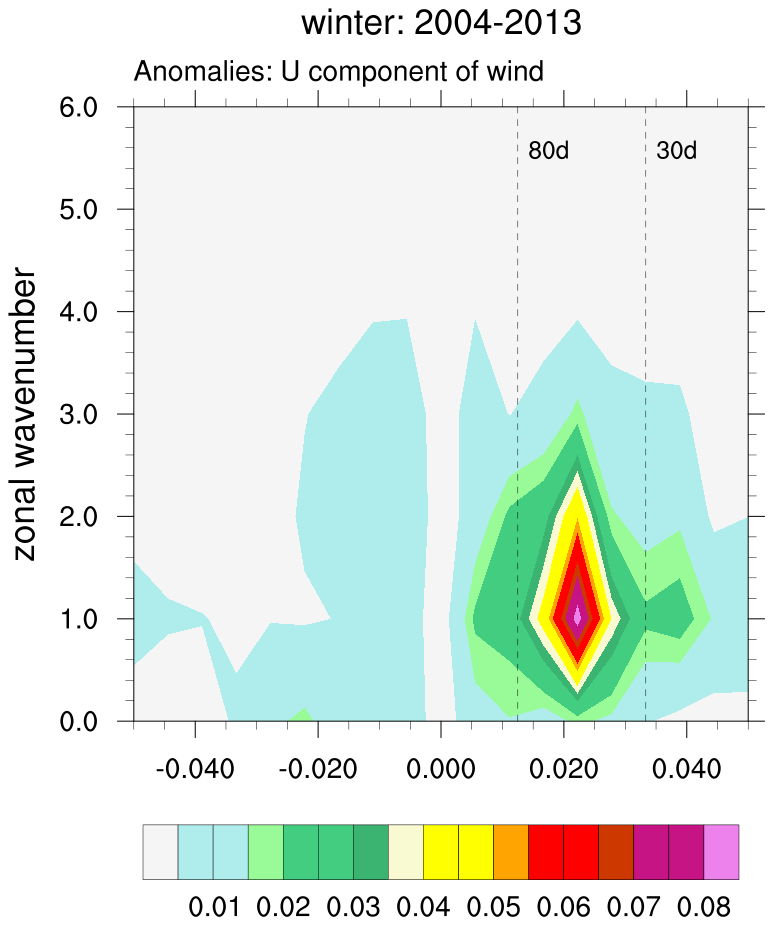
\includegraphics[width=6cm]{figures/obs-u850-wavefreq-winter.png}
\caption{MJO观测冬季U850波谱场}
\end{minipage}
\begin{minipage}[t]{0.48\textwidth}
\centering
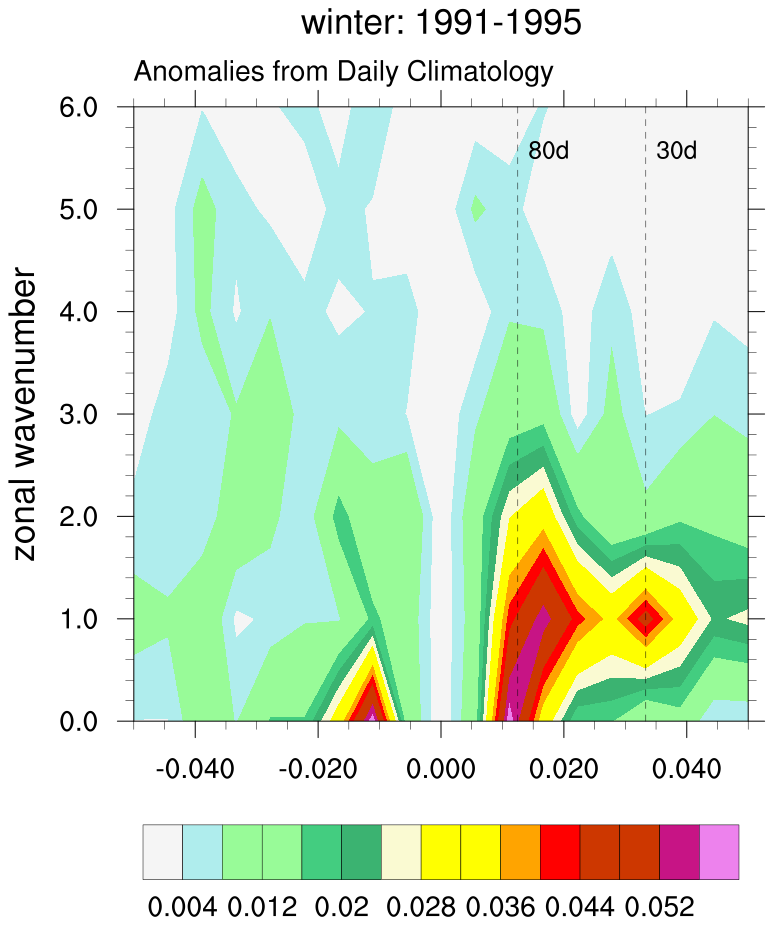
\includegraphics[width=6cm]{figures/cntl-u850-wavefreq-winter.png}
\caption{MJO控制预报的冬季U850波谱场}
\end{minipage}
}
\subfigure{
\begin{minipage}[t]{0.48\textwidth}
\centering
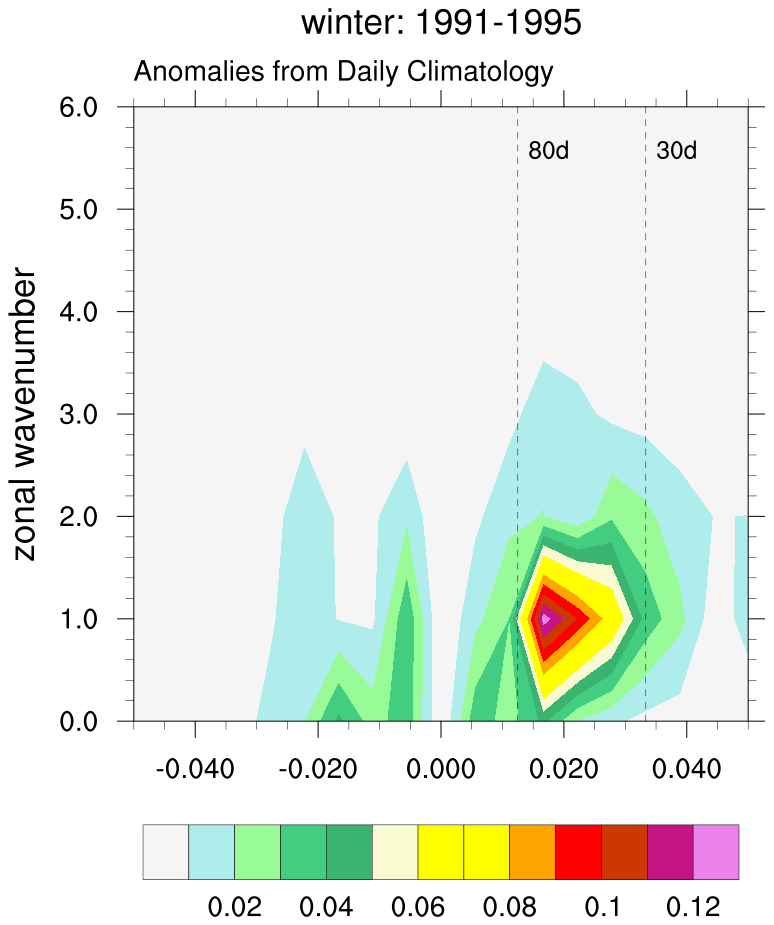
\includegraphics[width=6cm]{figures/runstandrad-u850-wavefreq-winter.png}
\caption{MJO优化参数后的冬季U850波谱场}
\end{minipage}
}
\end{figure}

\begin{figure}[H]
\label{8phase-lon}
\centering
\subfigure{
\begin{minipage}[t]{0.48\textwidth}
\centering
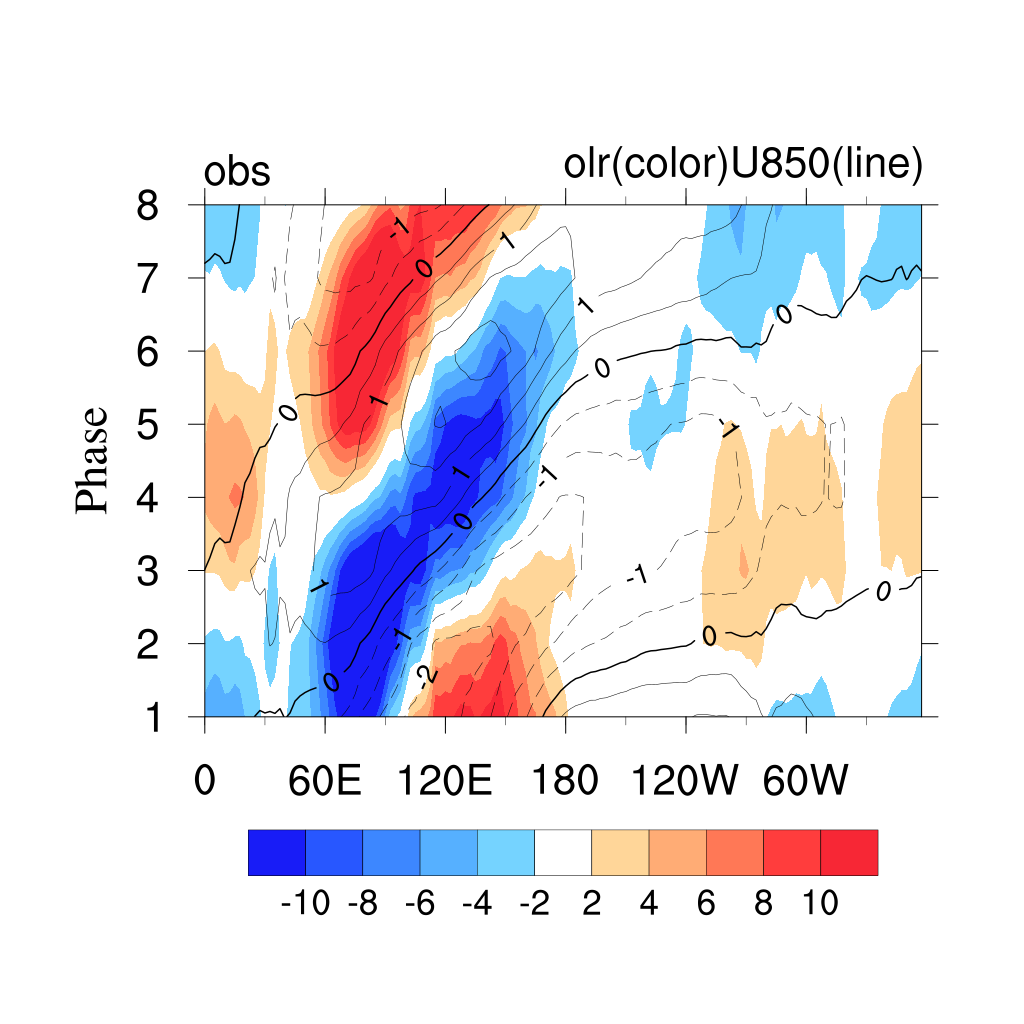
\includegraphics[width=8cm]{figures/obs-phase-lon.png}
\caption{MJO观测8位相合成图}
\end{minipage}
\begin{minipage}[t]{0.48\textwidth}
\centering
\includegraphics[width=8cm]{figures/cntl-phase-lon.png}
\caption{MJO控制预报的8位相合成图}
\end{minipage}
}
\subfigure{
\begin{minipage}[t]{0.48\textwidth}
\centering
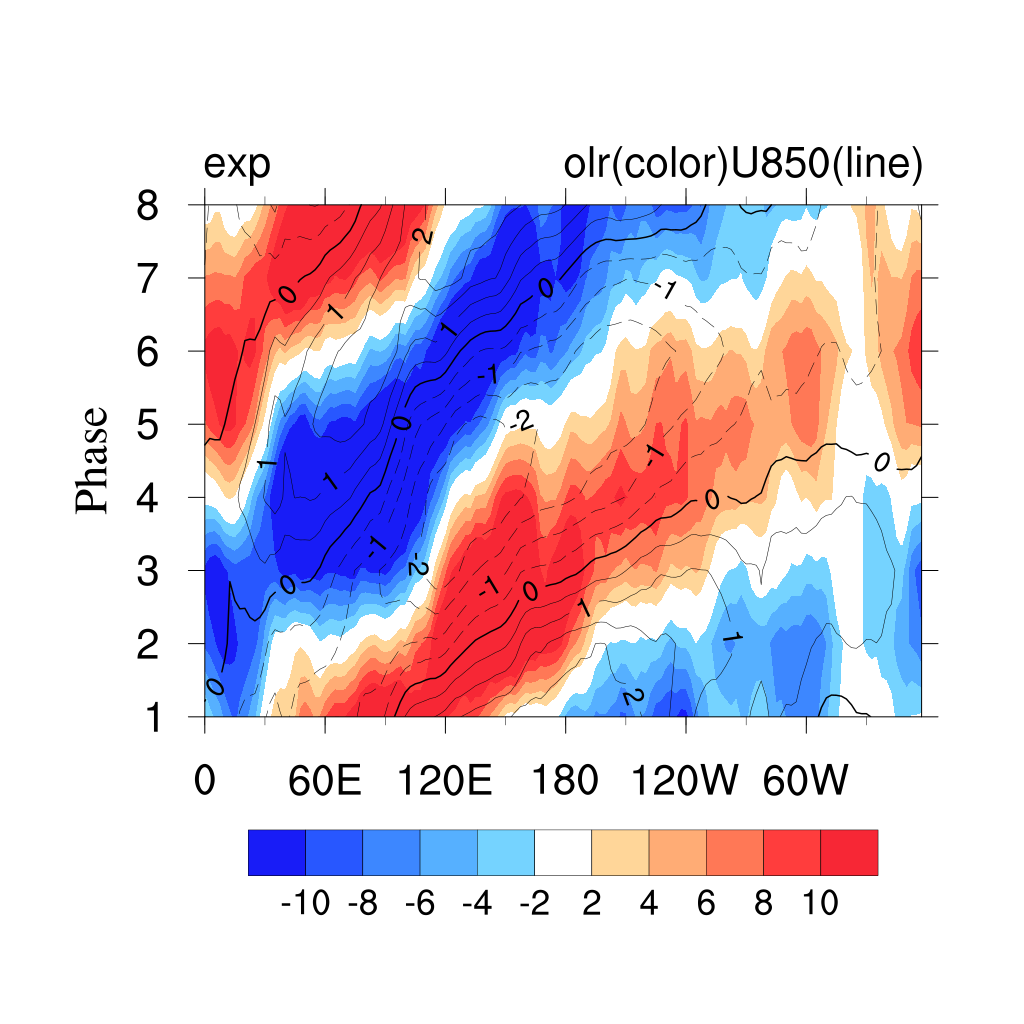
\includegraphics[width=8cm]{figures/runstandrad-phase-lon.png}
\caption{MJO改进参数后的8位相合成图}
\end{minipage}
}
\end{figure}

 \begin{figure}[H]
\centering
\begin{minipage}[t]{0.48\textwidth}
\centering
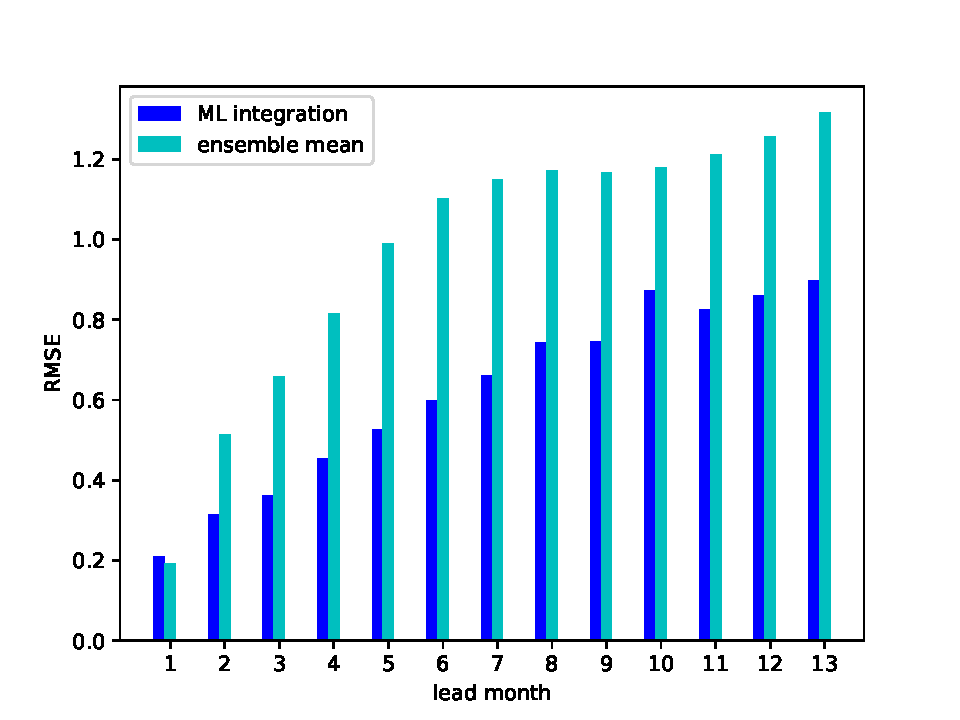
\includegraphics[width=8cm]{figures/RMSEensega.pdf}
%\caption{RMSE对比}
\end{minipage}
\begin{minipage}[t]{0.48\textwidth}
\centering
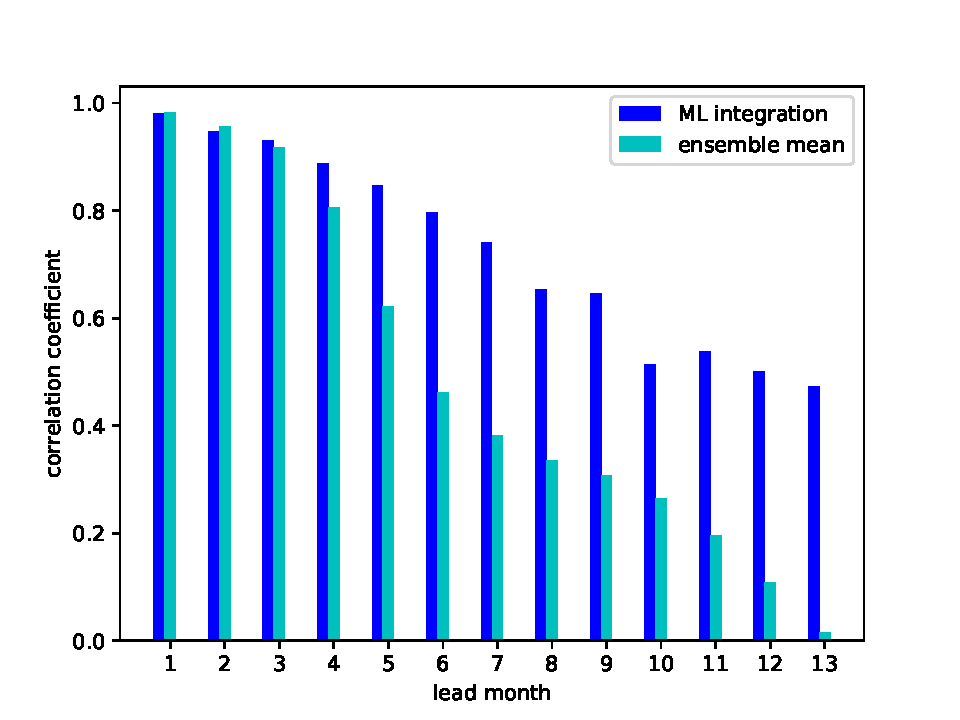
\includegraphics[width=8cm]{figures/RMSEensegacorr.pdf}
%\caption{相关系数对比}
\end{minipage}
\caption{机器学习修正方法与集合平均集成结果对比}
\end{figure}

\begin{figure}[H] % use float package if you want it here
  \centering
  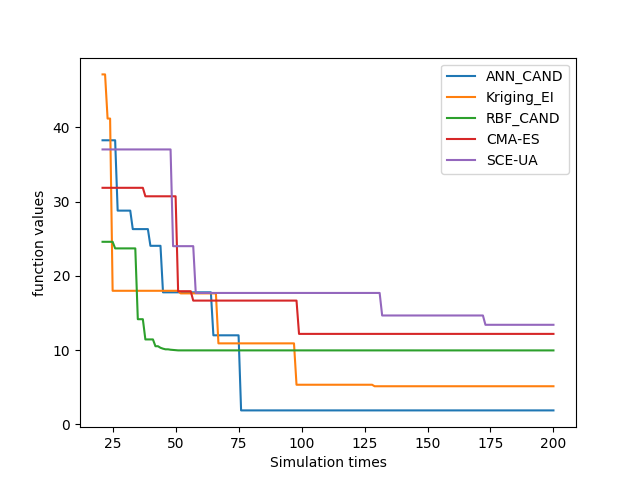
\includegraphics[scale=0.6]{figures/all_Rast4.png}
  \caption{单目标优化算法在Rastrigin函数上的优化结果}
  \label{fig:xfig1}
\end{figure}

\begin{figure}[H] % use float package if you want it here
  \centering
  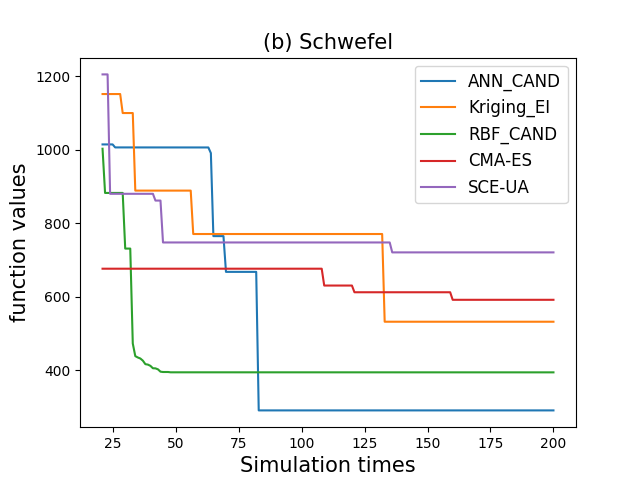
\includegraphics[scale=0.6]{figures/all_schw4.png}
  \caption{单目标优化算法在Schwefel函数上的优化结果}
  \label{fig:xfig1}
\end{figure} 

\begin{figure}[H] % use float package if you want it here
\label{prectresult}
  \centering
  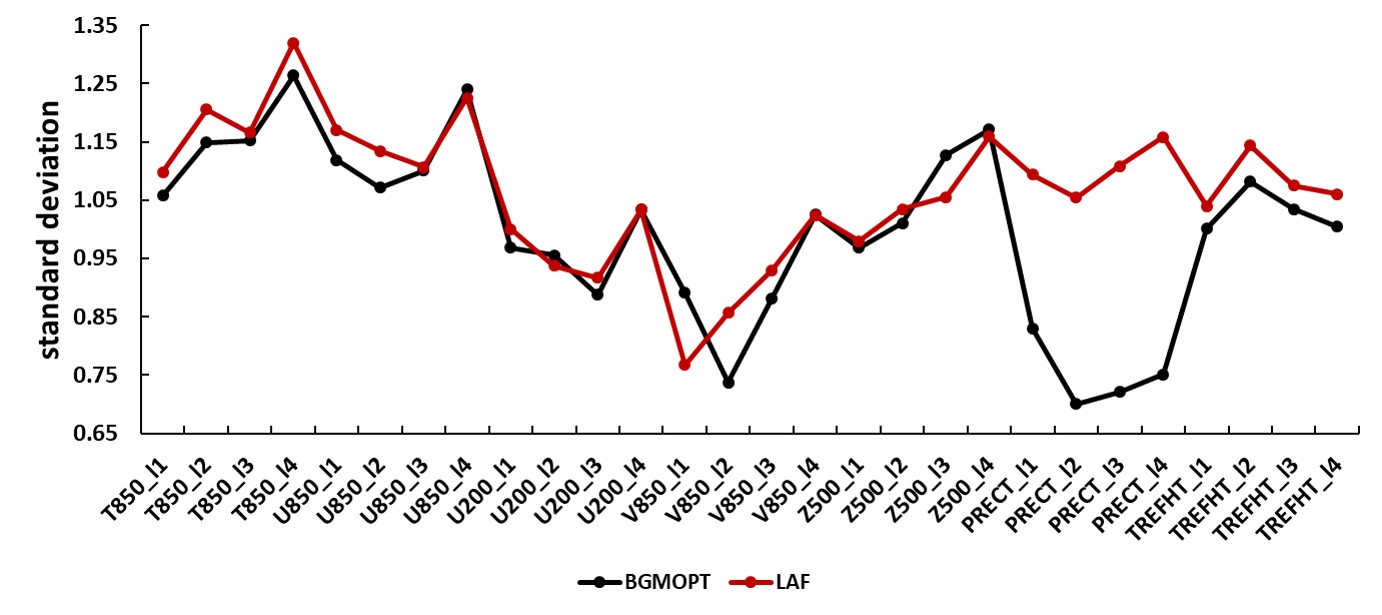
\includegraphics[scale=0.6]{figures/allvar-std.jpg}
  \caption{集合方法针对降水RMSE结果对比}
  \label{fig:xfig1}
\end{figure} 

\begin{figure}[H] % use float package if you want it here
\label{prectresult}
  \centering
  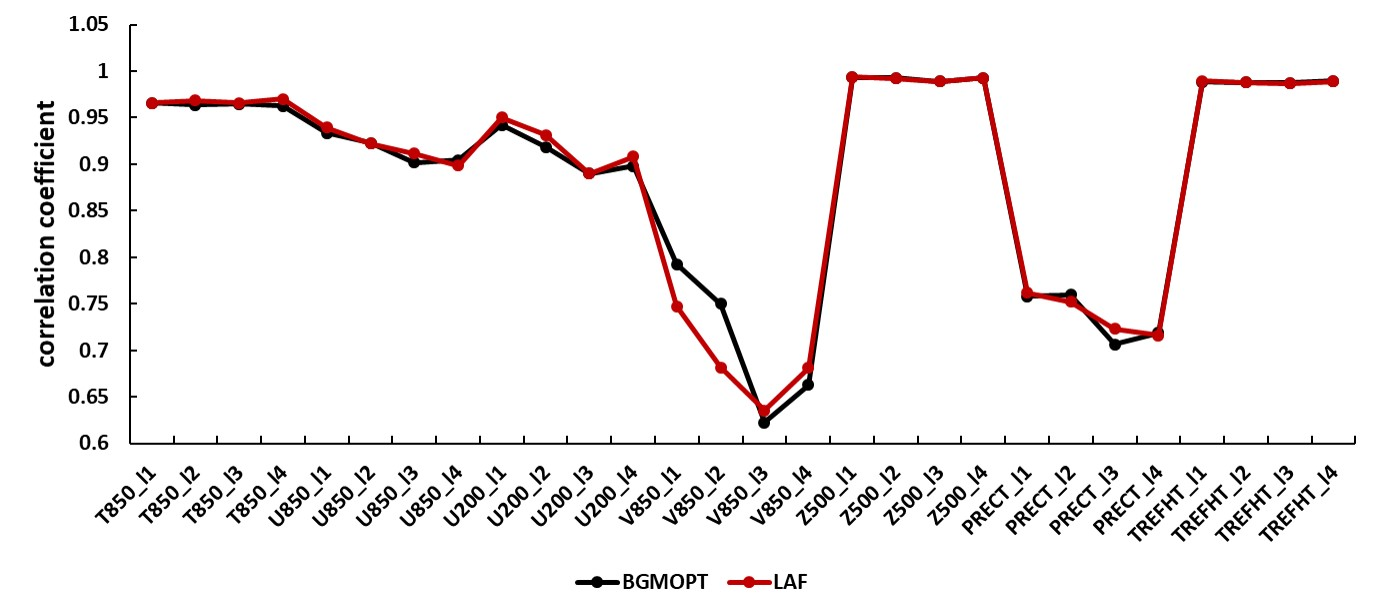
\includegraphics[scale=0.6]{figures/allvar_coef.jpg}
  \caption{集合方法针对降水correlation coefficient结果对比}
  \label{fig:xfig1}
\end{figure} 

\begin{figure}[H] % use float package if you want it here
\label{prectresult}
  \centering
  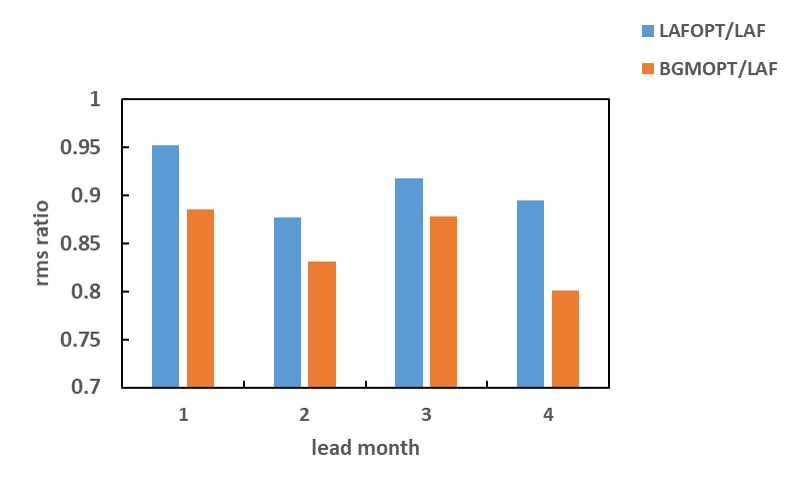
\includegraphics{figures/rmse-precip.jpg}
  \caption{集合方法针对降水RMSE结果对比}
  \label{fig:xfig1}
\end{figure} 

\begin{figure}[H] % use float package if you want it here
\label{prectresult}
  \centering
  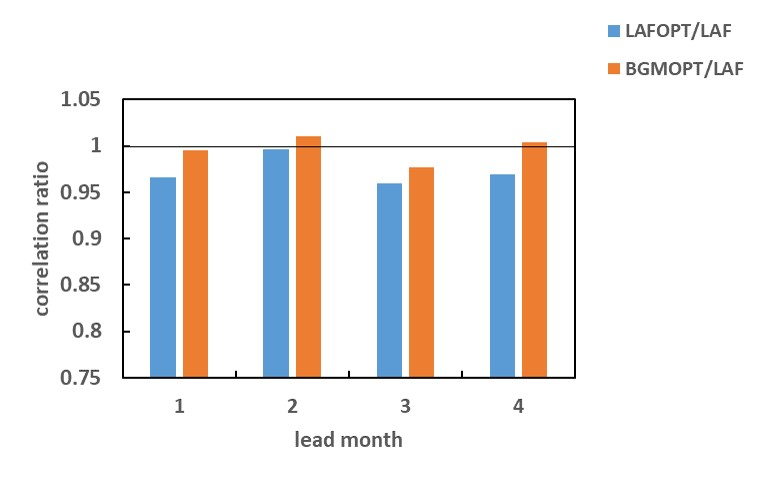
\includegraphics{figures/corr-precip.jpg}
  \caption{集合方法针对降水correlation coefficient结果对比}
  \label{fig:xfig1}
\end{figure} 

\begin{figure}[H] % use float package if you want it here
\label{Fig:easmresut}
 \centering
 \subfigure[集合集成方法的RMSE比较]{
 \centering
    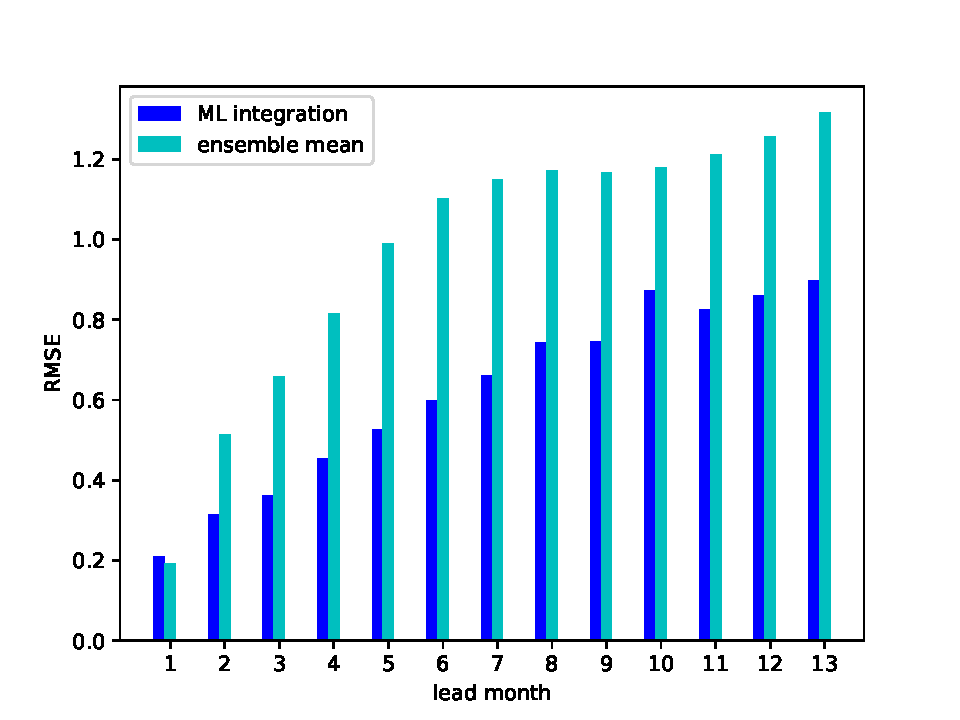
\includegraphics[scale=0.55]{figures/RMSEensega.pdf}
}

 \subfigure[集合集成方法的相关系数的比较]{
 \centering
     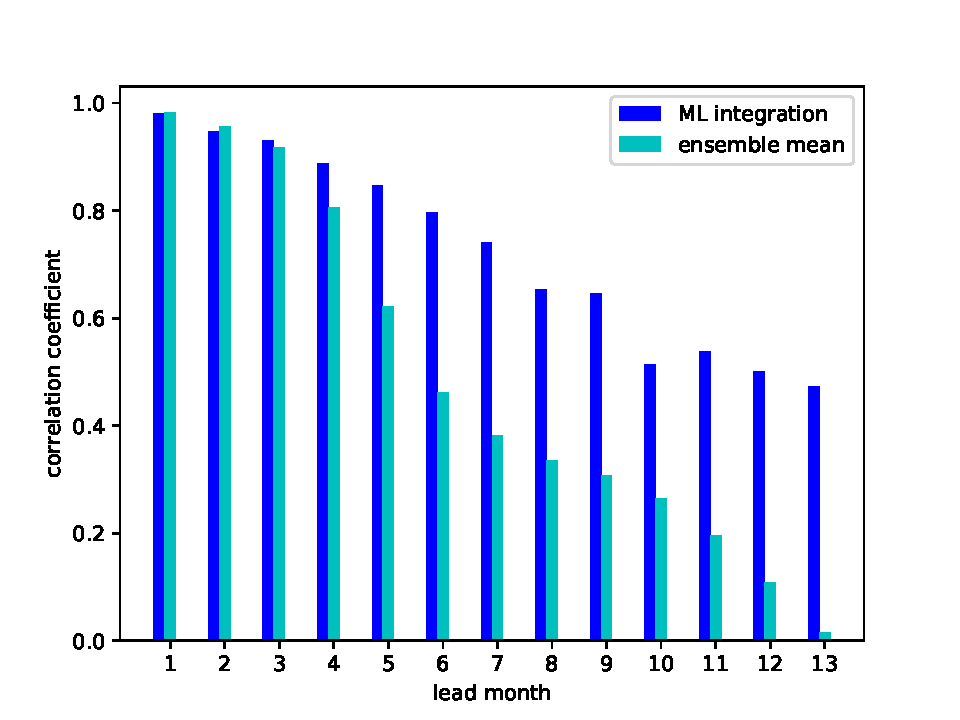
\includegraphics[scale=0.5]{figures/RMSEensegacorr.pdf}
 }
 \caption{机器学习修正方法与集合平均集成结果对比}
 \end{figure}

\begin{figure}[H] % use float package if you want it here
  \centering
  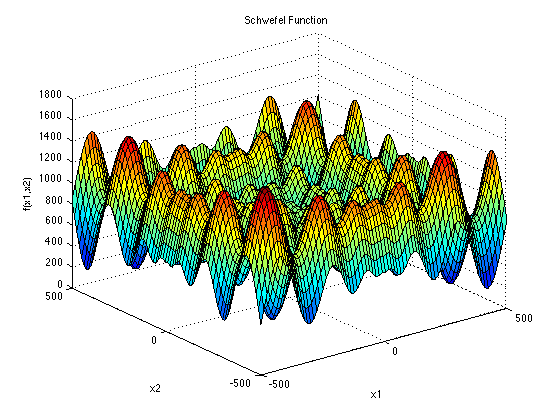
\includegraphics[scale=0.5]{schwef.png}
  \caption{Schwefel函数二维空间图}
  \label{fig:xfig1}
\end{figure}

\begin{figure}[H] % use float package if you want it here
  \centering
  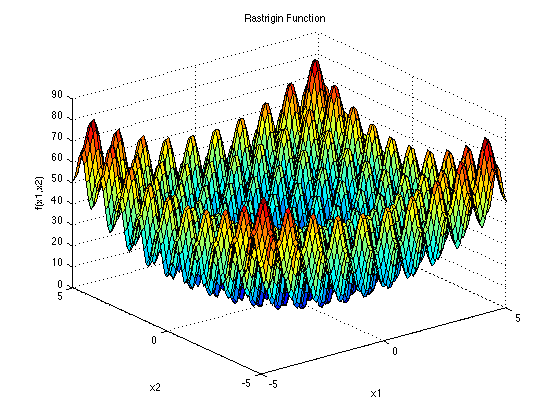
\includegraphics[scale=0.5]{rastr.png}
  \caption{Rastrigin函数二维空间图}
  \label{fig:xfig1}
\end{figure}

\begin{figure}[H] % use float package if you want it here
  \centering
  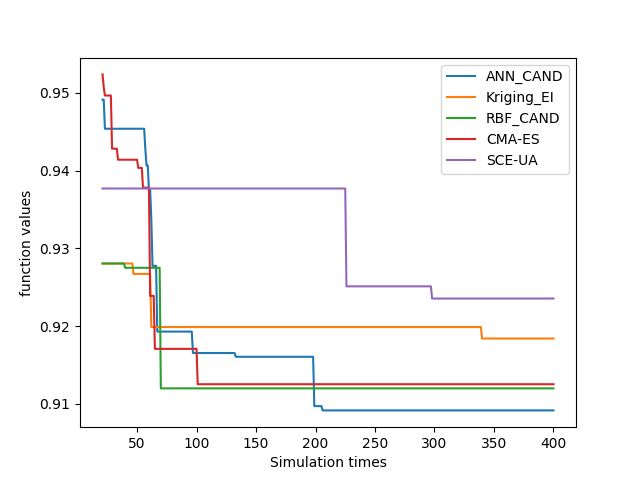
\includegraphics[scale=0.6]{figures/all_scam_new.png}
  \caption{单目标优化算法在TWPSCAM上的优化结果}
  \label{fig:xfig1}
\end{figure} 

\begin{figure}[H] % use float package if you want it here
  \centering
  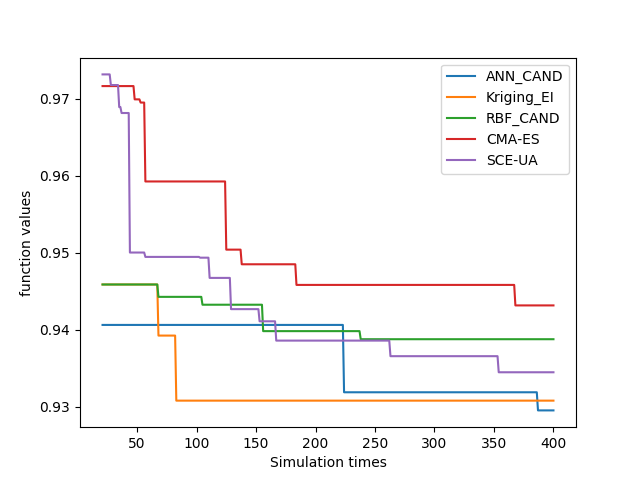
\includegraphics[scale=0.6]{figures/all_scam_ARW.png}
  \caption{单目标优化算法在MPSCAM函数上的优化结果}
  \label{fig:xfig1}
\end{figure}

\begin{figure}[H] % use float package if you want it here
\label{prectresult}
  \centering
  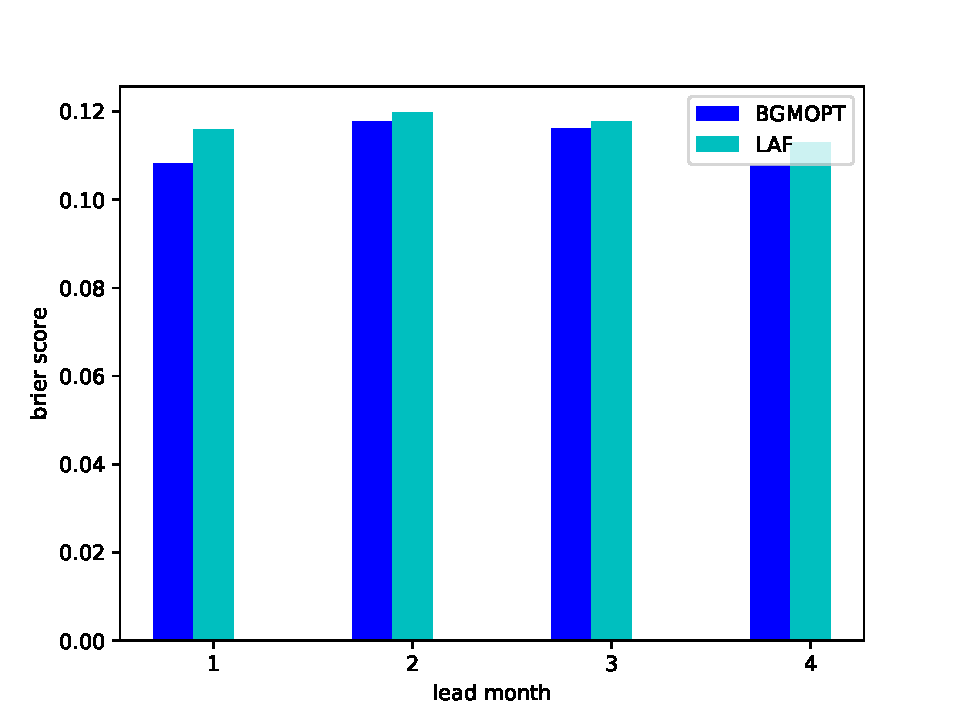
\includegraphics[scale=0.55]{figures/brier.pdf}
  \caption{集合方法关于降水Brier评分结果}
  \label{fig:xfig1}
\end{figure}


\begin{figure}[H] % use float package if you want it here
\label{prectresult}
  \centering
  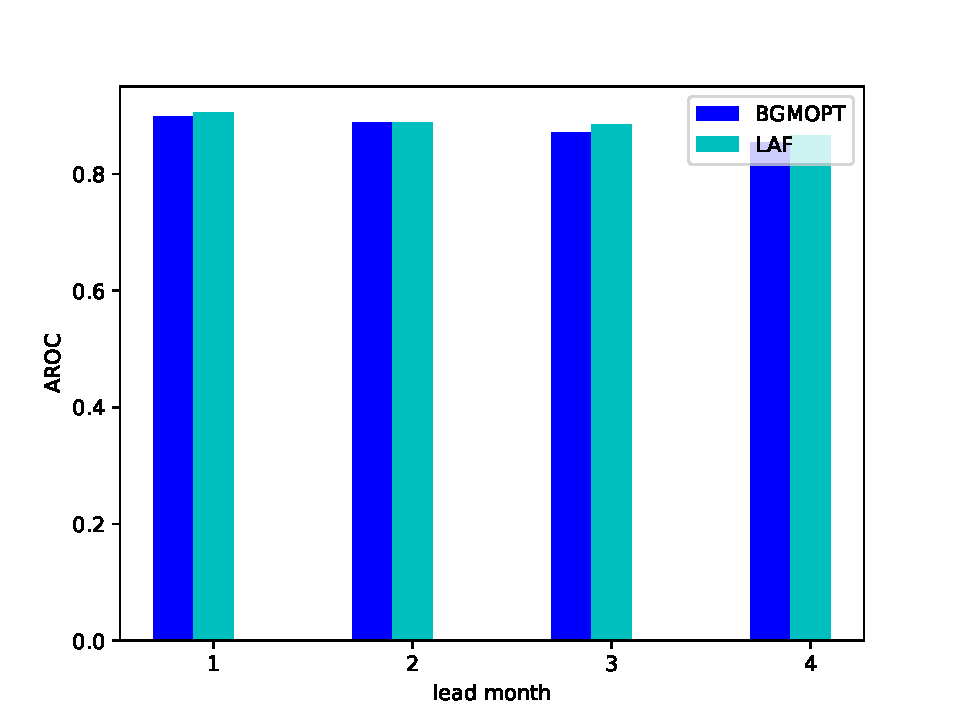
\includegraphics[scale=0.55]{figures/AROC.pdf}
  \caption{集合方法关于降水AROC的评比结果}
  \label{fig:xfig1}
\end{figure}

另外一个经常用来作为集合概率预报的评价的方法是相对操作特征面积ROCA(Relative Operating Characteristics Area)其意义是以假警报率为横坐标,以命中率为纵坐标的ROC曲线下的面积,面积越大则说明预报技巧越高。


\begin{figure}[H] % use float package if you want it here
  \centering
  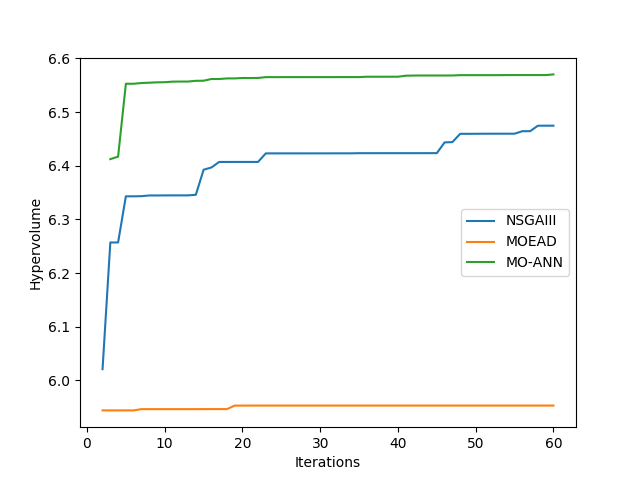
\includegraphics[scale=0.6]{TWPMOnew.png}
  \caption{TWP-ICE单柱大气模型上多目标算法的hypervolume}
  \label{fig:xfig1}
\end{figure} 
\begin{figure}[H] % use float package if you want it here
  \centering
  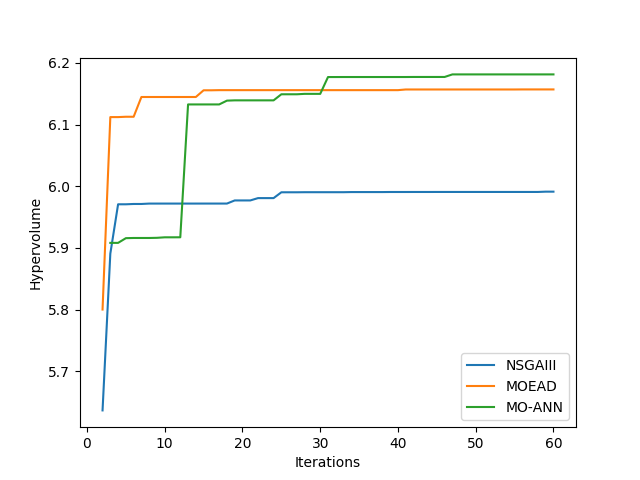
\includegraphics[scale=0.6]{figures/ARW-MO.png}
  \caption{M-PACE单柱大气模型上多目标算法的hypervolume}
  \label{fig:xfig1}
\end{figure} 

\begin{figure}[H] % use float package if you want it here
  \centering
  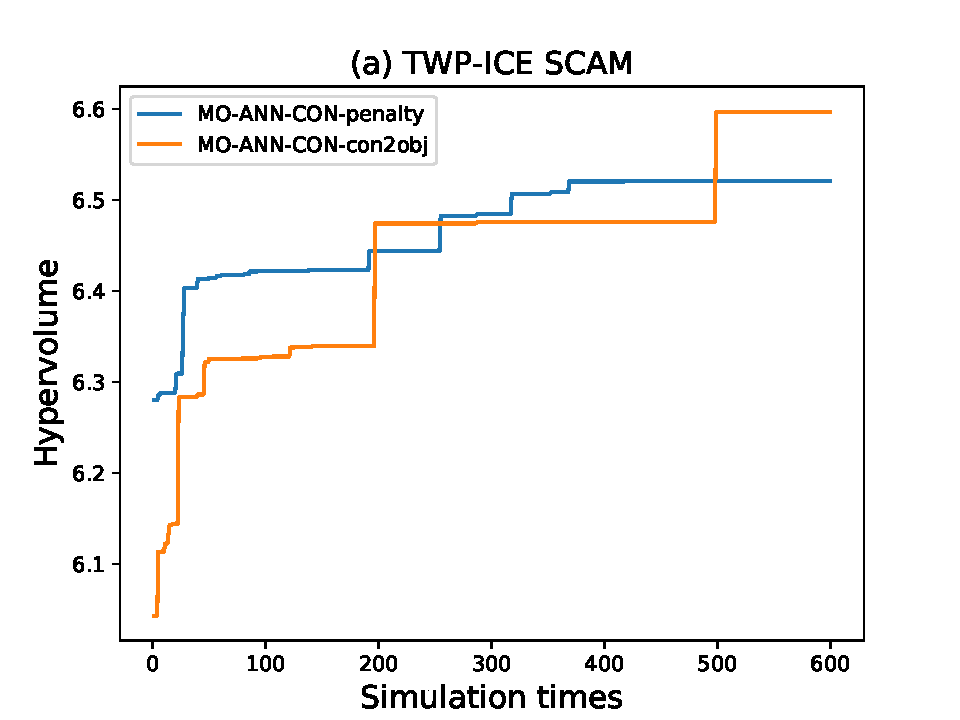
\includegraphics[scale=0.6]{figures/twpconstraint.pdf}
  \caption{TWP-ICE单柱大气模型上有约束多目标算法的hypervolume}
  \label{fig:xfig1}
\end{figure} 
\begin{figure}[H] % use float package if you want it here
  \centering
  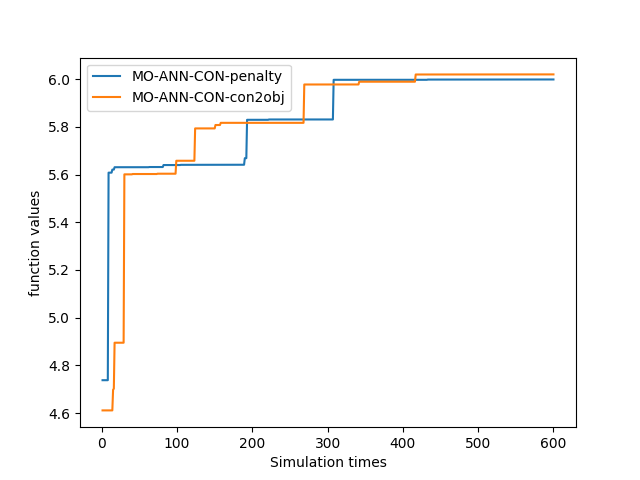
\includegraphics[scale=0.6]{arwconstaint.png}
  \caption{M-PACE单柱大气模型上有约束多目标算法的hypervolume}
  \label{fig:xfig1}
\end{figure}

其典型的例子有基于Kriging模型的EGO(Efficient
Global Optimization)算法~\cite{mohammadi2016kriging}。



\section{面向气候系统模式参数的代理模式优化实现}
\subsection{参数优化准备工作}

参数优化准备工作

1.气候系统模式的移植与验证

2.气候系统模式参数的抽取与验证

\subsection{总体设计}
1.优化问题定义部分。此部分定义问题的输入维度,参数的取值范围,所需要优化的问题。对于气候系统模式的来说,需要优化的是针对某一个评价标准的模式性能表现。这里需要自动化的参数匹配,模式运行和结果评估。如果是多目标优化问题需要利用Hypervolume等指标综合评价非支配解的优劣。

2.代理模式的建立部分。获取参数值与其对应的气候系统模式评价结果样本时需要将样本用来训练代理模式。此模块有MLP的具体实现过程,MLP的总层数以及每一层的隐元个数,激活函数和学习率等超参数的设置。

(1)模型的建立
(2)模型的训练与测试
(2)超参的调优
(3)模型的预测

3.优化算法的优化策略部分。此部分主要是各个代理模式优化算法的最优样本选择策略。在单目标、多目标、有约束优化的实现过程中有些细节上的调整。

4.优化总流程的调度。此部分将面向气候系统模式参数优化的每一个流程串联在一起,包括从一开始的拉丁超立方采样到代理模式的训练再到新的采样点的选取等。
(1)采样
(2)
(2)初始代理模型拟合
(3)新采样点的获取
(4)新采样点的评估

本文中所使用的多层感知机学习率为0.01,隐含层为2,每层隐元数为200,激活函数分别都为sigmoid,输出层的激活函数为Relu,输入层神经元的个数为所需优化参数的维度,输出层神经元的个数为优化目标的个数。在这样一个基础的多层感知机上利用当前所有样本,通过反向传播算法更新神经网络的权重,使其能够很好的拟合当前所有样本。

\begin{figure}[H] % use float package if you want it here
  \centering
  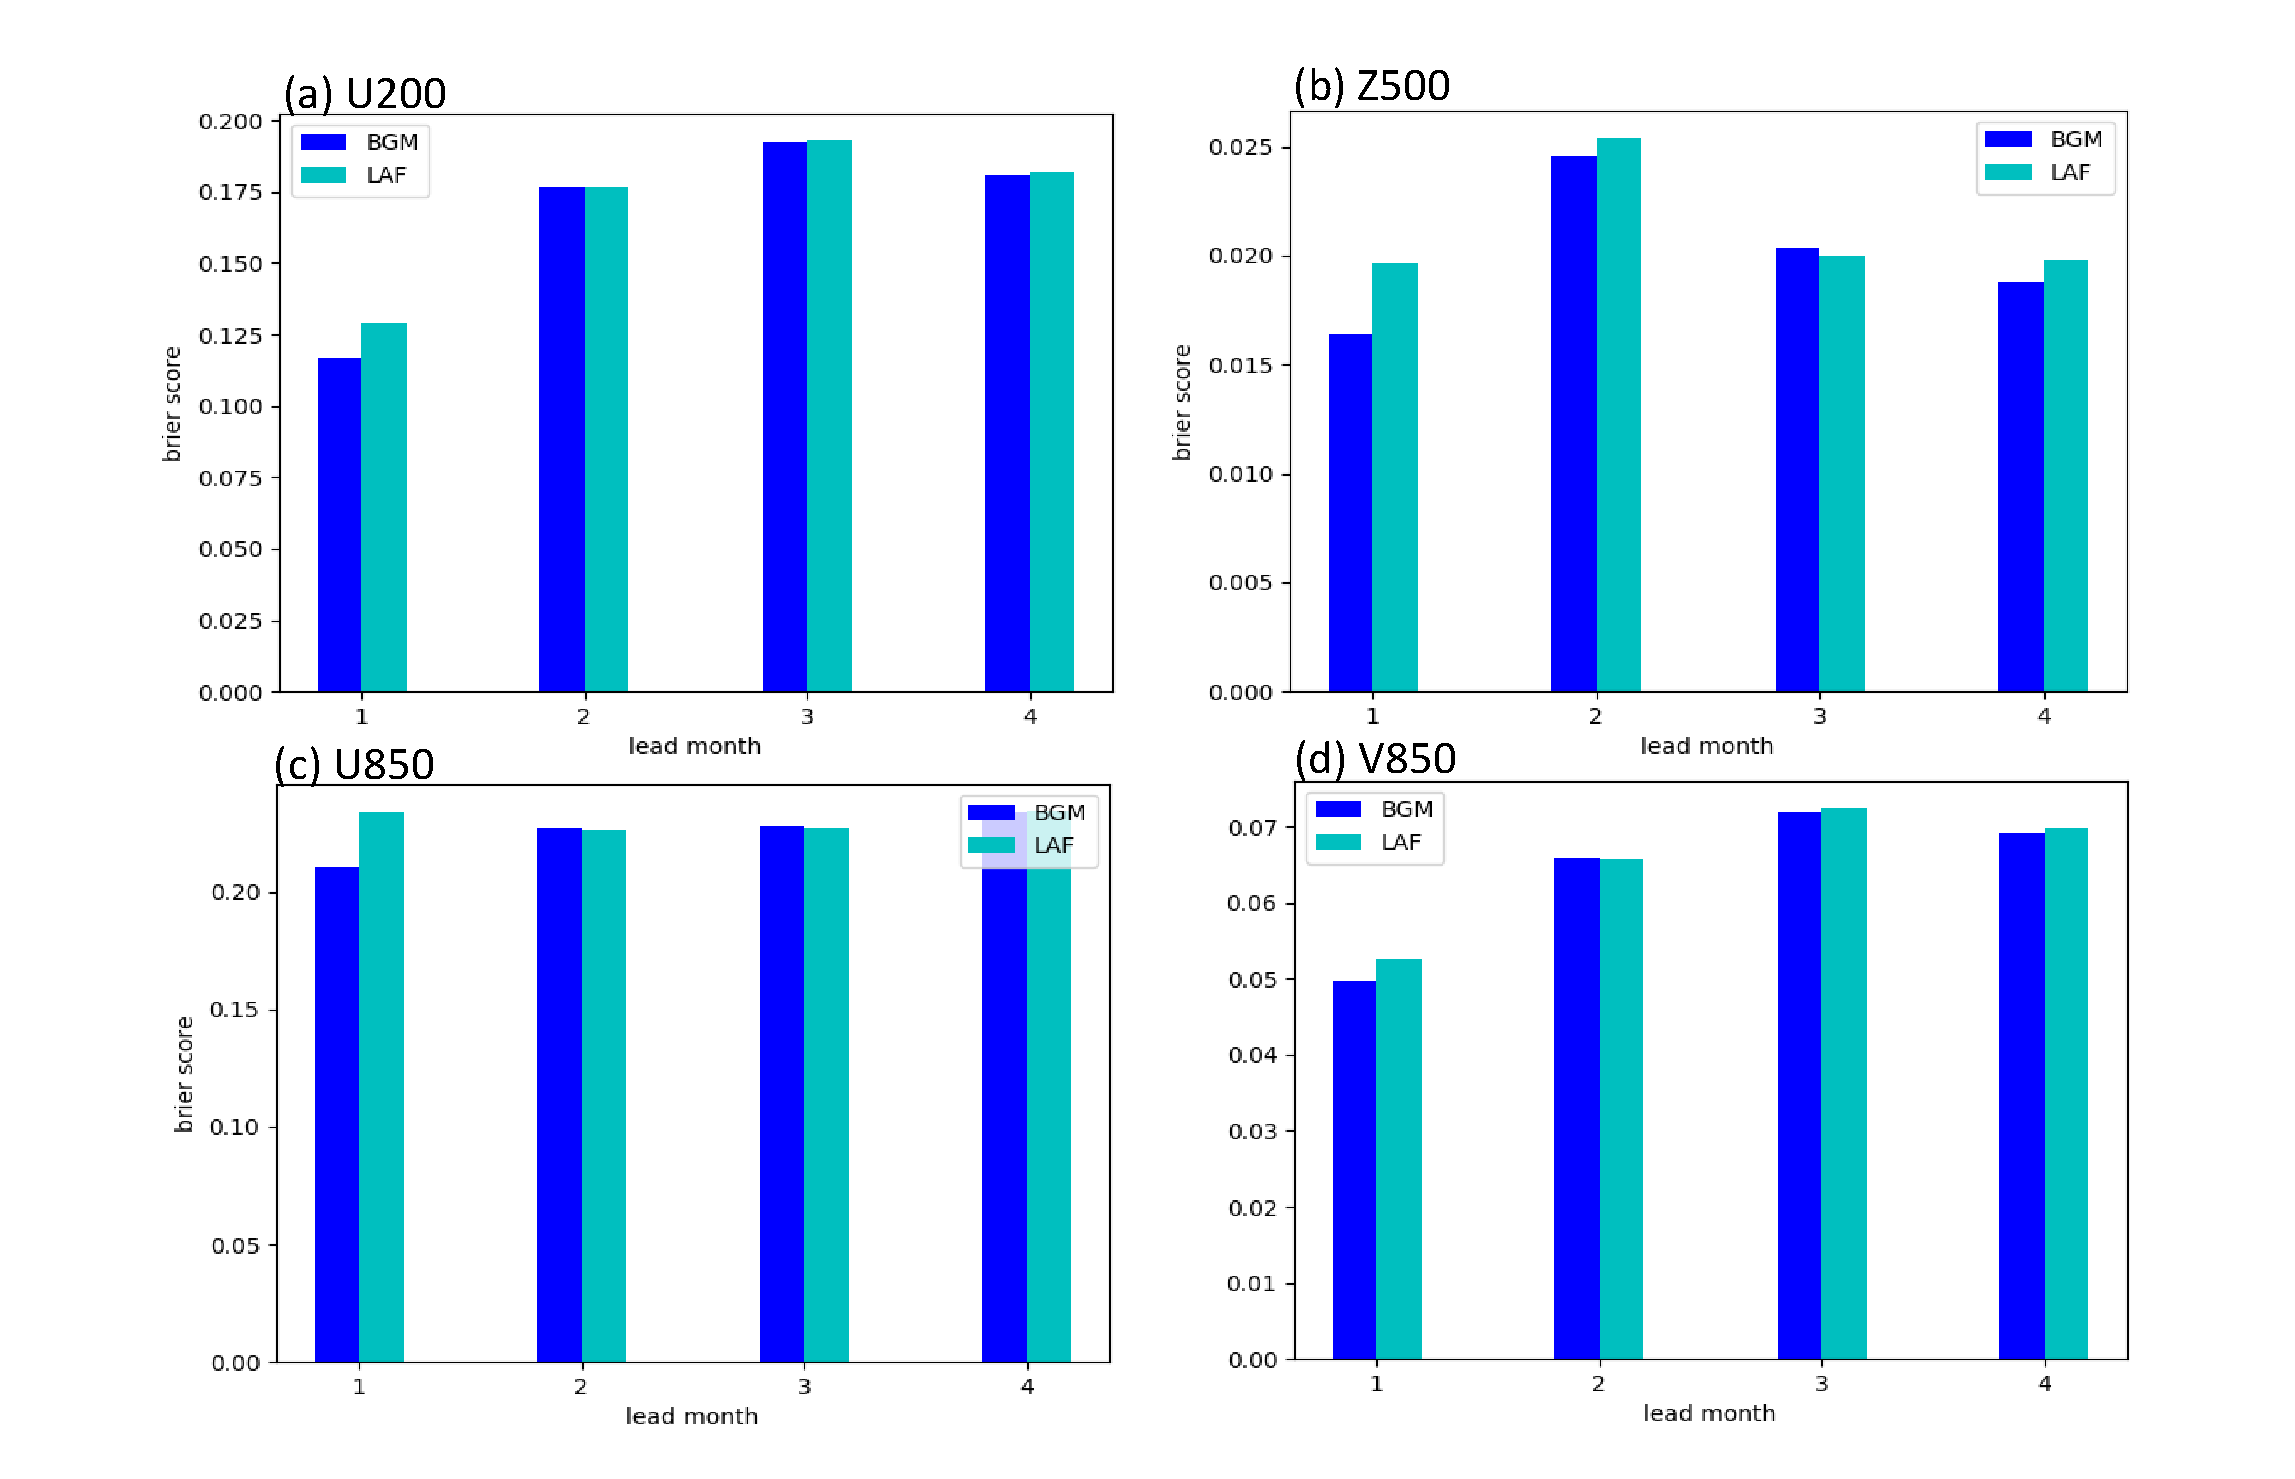
\includegraphics[scale=0.45,trim=60 10 20 10,clip]{figures/allBrier.pdf}
  \caption{U200,Z500,U850,V850全球平均BS评分}
  \label{fig:BS}
\end{figure}




\begin{figure}[H] % use float package if you want it here
  \centering
  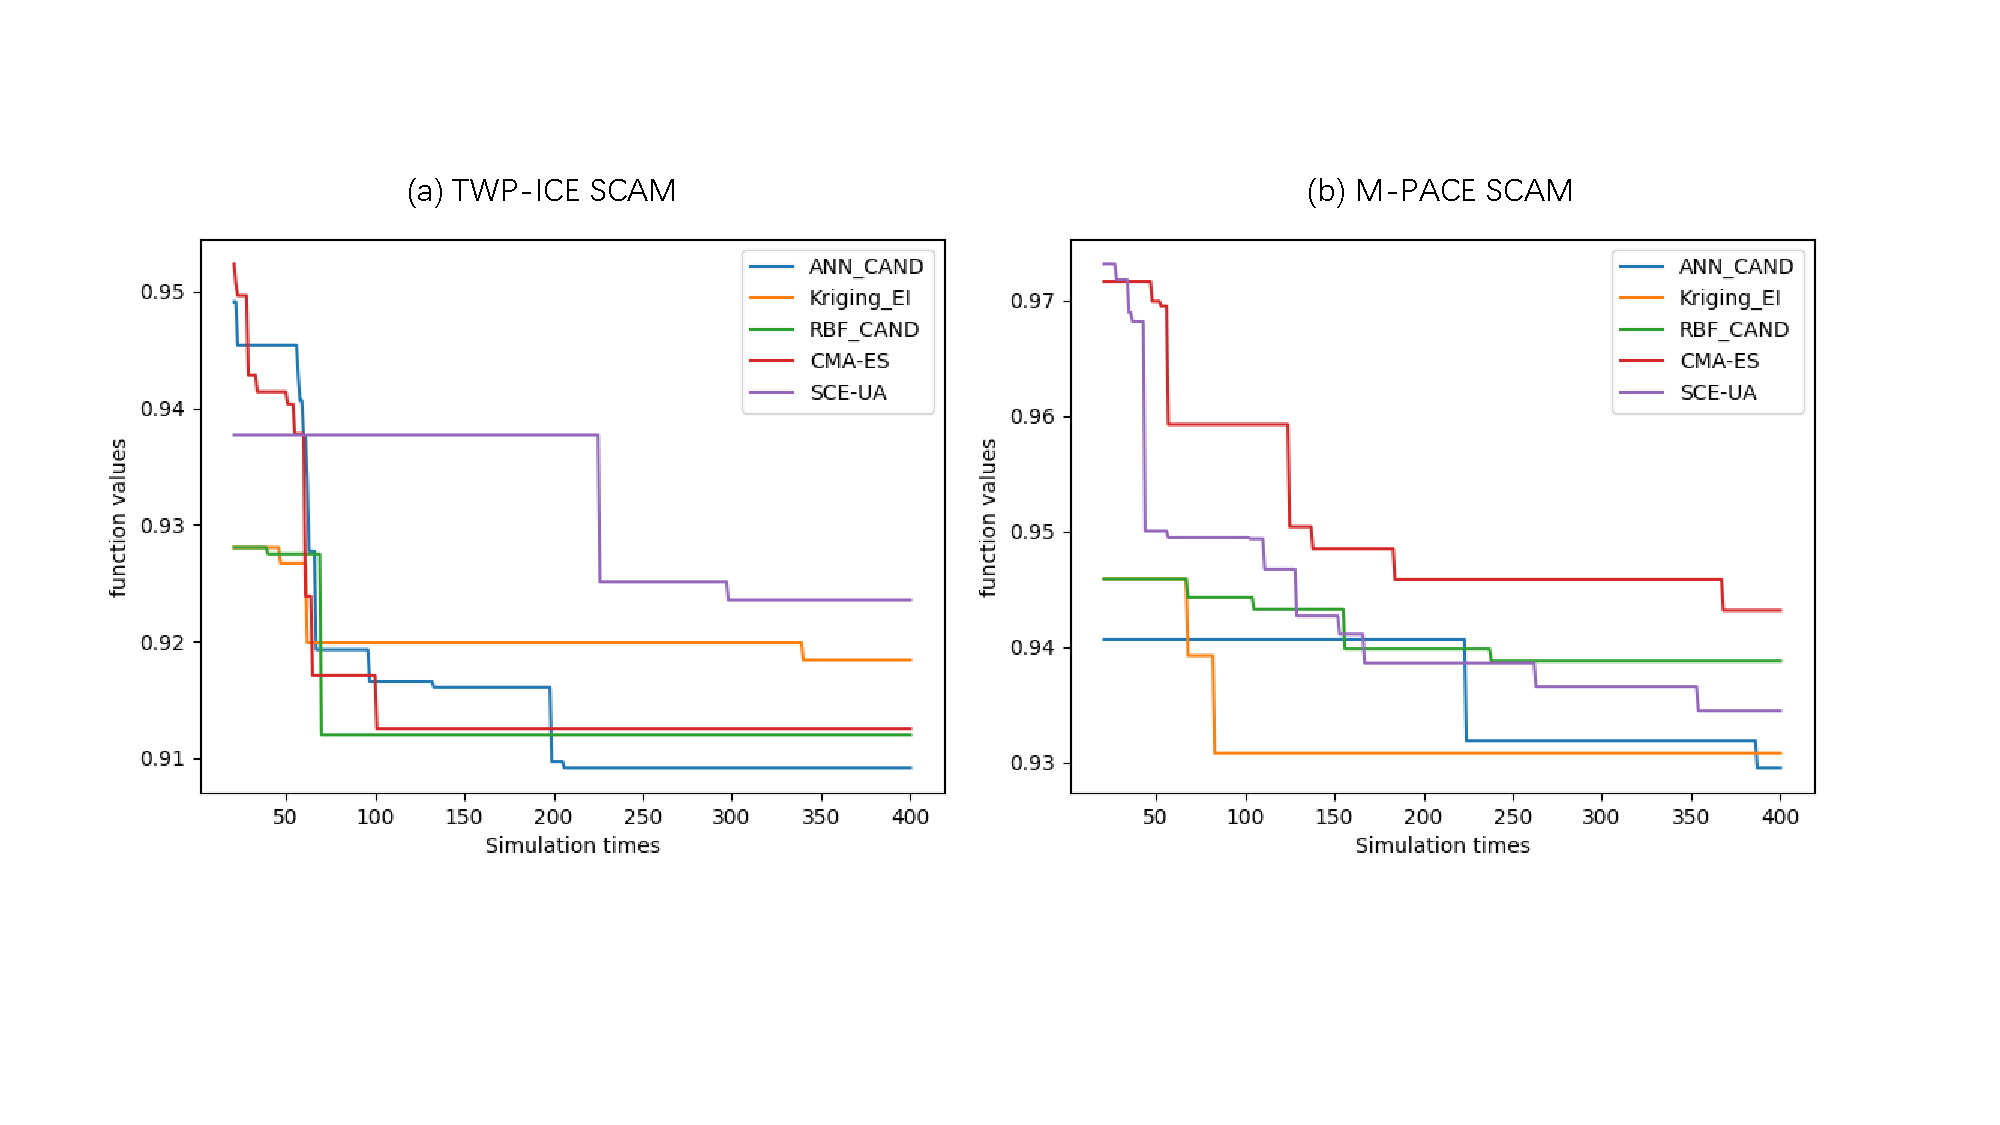
\includegraphics[scale=0.5,trim=10 100 10 85,clip]{figures/soallscam.pdf}
  \caption{单目标优化算法在TWP-ICE和M-PACE单柱大气模式上的优化结果}
  \label{fig:soscam}
\end{figure}

\begin{figure}[H] % use float package if you want it here
  \centering
  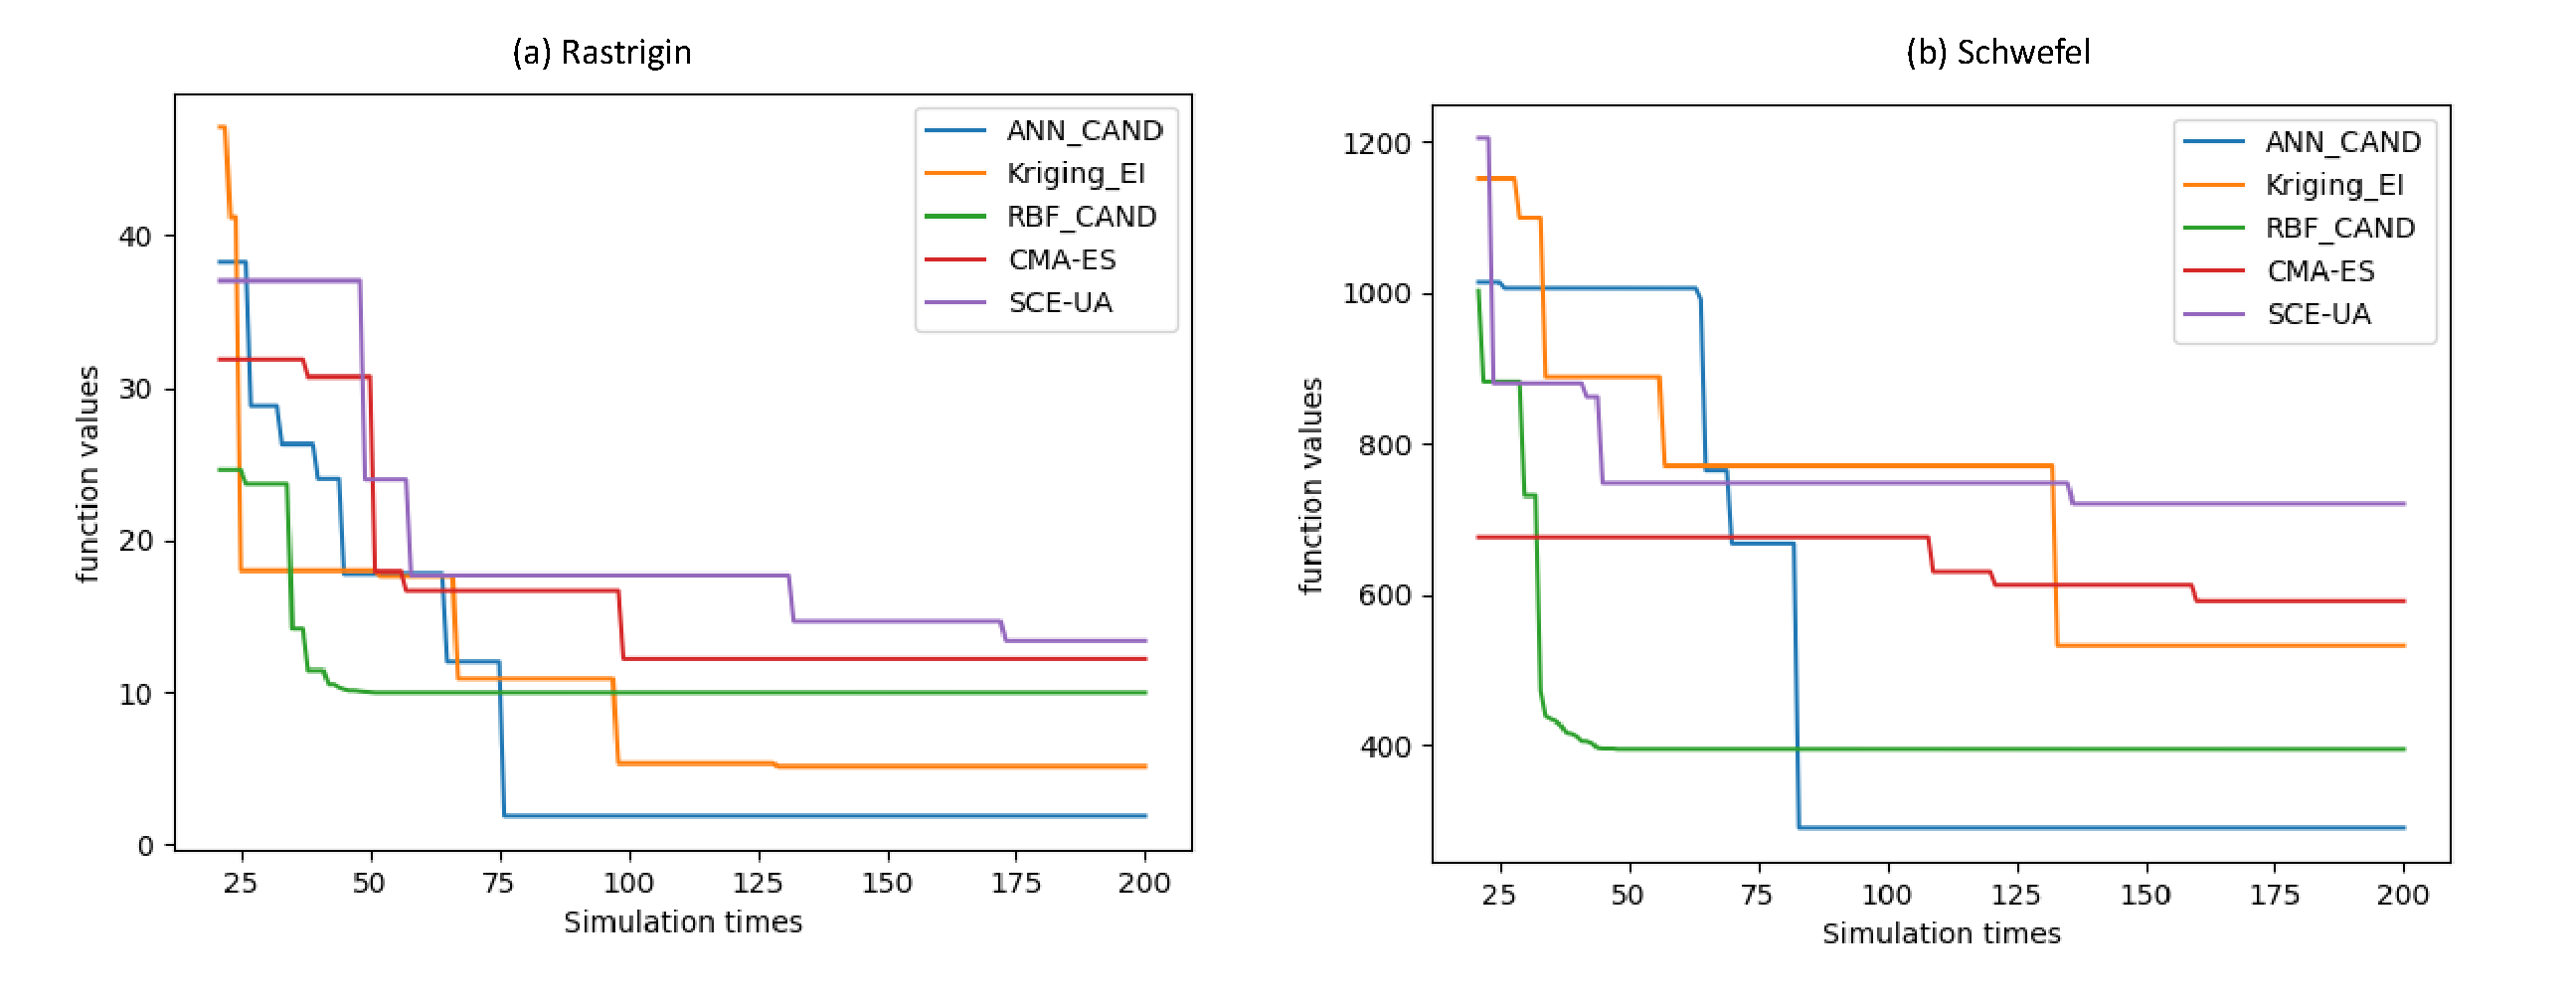
\includegraphics[scale=0.35,trim=0 10 10 10,clip]{figures/SOallfuction.pdf}
  \caption{单目标优化算法在Rastrigin和Schwefel函数上的优化结果}
  \label{fig:sofuction}
\end{figure}









